\documentclass{article}
% Comment the following line to NOT allow the usage of umlauts
\usepackage[utf8]{inputenc}
\usepackage[french]{babel}
\usepackage[a4paper, total={6in, 8in}]{geometry}
\usepackage{graphicx}
\usepackage{afterpage}
\usepackage{xcolor}
\usepackage[sfdefault,light]{roboto}
\usepackage[T1]{fontenc}
\usepackage{sectsty}
\usepackage[titles]{tocloft}
\usepackage{eso-pic}
\usepackage{fancyhdr}
\usepackage{pagecolor}
\usepackage{subfig}

\definecolor{background}{HTML}{13181e}
\definecolor{green}{HTML}{32bba9}
\definecolor{greendark}{HTML}{16a085}


\sectionfont{\color{green}}  % sets colour of sections
\subsectionfont{\color{green}}  % sets colour of sections
\subsubsectionfont{\color{green}}
\color{background}
% Start the document
\begin{document}

\makeatletter
    \begin{titlepage}
        \begin{center}
            \pagecolor{background}
            \color{white}
            
\includegraphics[width=0.5\linewidth]{assets/shape.png}\\[10ex]
            {\huge \bfseries BilleGateCoin - BGC}\\[2ex] 
            {\LARGE Scattered Corporation}\\[10ex]
            
            {\huge \bfseries RAPPORT DE SOUTENANCE}\\[5ex]
            \large{réalisé par\\[2ex]aurele.oules  •  leo.gervoson  •  raphael.brenn}\\[16ex] 
            {\large Projet EPITA 2020}
        \end{center}
    \end{titlepage}
\makeatother
\thispagestyle{empty}

\newpage
\begin{center}
\color{white}
\tableofcontents
\end{center}
\newpage
\pagecolor{white}
\sectionfont{\color{greendark}}  % sets colour of sections

\fancyhf{}
\renewcommand{\headrulewidth}{0pt}
\renewcommand{\footrulewidth}{1pt}
\newcommand\bold[1]{\textcolor{green}{\bfseries{#1}}}
\newcommand\boldblack[1]{\textcolor{background}{\bfseries{#1}}}
\renewcommand{\footrule}{\hbox to\headwidth{\color{green}\leaders\hrule height \footrulewidth\hfill}}

\lfoot{%
   \smash{%  % hide vertical stretch of the following content
    \parbox[b]{\textwidth}{%
    \raggedright
    \footnotesize
    
\includegraphics[width=0.08\linewidth]{assets/shape.png}\\[-7ex]
    }%
   }%
}
\rfoot{\thepage}
\pagestyle{fancy}
\renewcommand\seriesdefault{l}

% Create a new 1st level heading
\section{Introduction}
BilleGateCoin est une plateforme décentralisée pour un jeu de billes.

\section{Génération du portefeuille}
Un portefeuille consiste d'une clé privée et d'une clé publique correspondante. Celui-ci permet de signer des contrats sur la plate-forme and remplace le système basique d'email/mot de passe.
La génération d'un portefeuille se fait en plusieurs étapes.

ECDSA est l'algorithme cryptographique utilsé par BGC pour signer les contrats.
BilleGateCoin utilise la courbe elliptique \bold{secp256k1}. Nous avons décidé d'utiliser le même algorithme de signature ainsi que la même courbe elliptique que le Bitcoin afin de pouvoir comparer nos résultats et également utiliser les normes déjà établies par la communauté.

La création d'une clé privée, clé publique et d'une adresse a été réalisé par \bold{Léo}.
\bold{Aurèle} a travaillé sur le chiffrement de la clé privée.

\subsection{Génération d'une clé privée}

Une clé privée est un nombre aléatoire compris entre $1$ et $2^{256} - 2^{32} - 2^{9} - 2^{8} - 2^{7} - 2^{6} - 2^{4} - 1$. Ce nombre doit être stocké de manière très sécurisée.

\subsection{Clé publique}
Une clé publique est dérivée de la clé privée avec l'algorithme ECDSA sur la courbe \bold{secp256k1}.

\subsection{Adresse}
Voici les étapes de génération d'une adresse.

\begin{itemize}
    \item Générer une clé privée
    \item Dériver la clé publique
    \item Réaliser un hash SHA-256 sur la clé publique
    \item Réaliser un hash RIPE-MD sur le hash SHA-256
    \item Ajouter l'octet de version devant le hash RIPE-MD (0x8A)
    \item Réaliser le hash double hash SHA-256 du hash RIPE-MD versionné
    \item Ajouter les 4 premiers octets du double hash (checksum) à la fin du hash RIPE-MD versionné
\end{itemize}

Exemple d'adresse: xZ7h1HUEcraAAHiJBqm1aDnr9nXJBh6yz8
\filbreak
\begin{verbatim}
public byte[] Address() {
    SHA256 sha526 = SHA256.Create();

    // Step 2: SHA256 hash
    byte[] hash = sha526.ComputeHash(PublicKey);

    // Step 3: RIPEMD-160 hash
    RIPEMD160 ripemd = RIPEMD160Managed.Create();
    byte[] ripemdHash = ripemd.ComputeHash(hash);
    
    // Step 4: Add version byte (0x00)
    byte[] versioned = new byte[ripemdHash.Length + 1];
    versioned[0] = Version;
    
    for (int i = 0; i < ripemdHash.Length; i++)
    {
        versioned[i + 1] = ripemdHash[i];
    }

    // Step 5 & 6: SHA256 twice
    hash = sha526.ComputeHash(versioned);
    hash = sha526.ComputeHash(hash);
    
    // Step 7 & 8: add trimmed hash at the end of the versioned hash
    byte[] address = new byte[ripemdHash.Length + 5];
    {
        int i = 0;
        for (; i < versioned.Length; i++)
        {
            address[i] = versioned[i];
        }
        for (int j = 0; j < 4; j++)
        {
            address[i + j] = hash[j];
        }
    }

    return address;
}
\end{verbatim}

\subsection{Chiffrement}
Une clé privée doit être stockée et chiffrée. Pour se faire, nous avons adopter l'algorithme de chiffrement \bold{AES}. Le porte-feuille est sauvegardé en tant que $wallet.dat$ et ne peut être déchiffré uniquement avec le mot de passe de l'utilisateur.

\section{Sérialisation}
La sérialisation est le codage d'une structure de données dans un format qui peut être lu et restitué plus tard. BilleGateCoin doit passer par ce processus de sérialisation afin de pouvoir stocker les différents contrats et block de la blockchain sur un disque dur, de manière compacte et optimisée.

\subsection{Contrats}
\subsubsection{Placement de billes}
Un placement de billes est une structure de données réutilisée dans plusieurs contrats. Un placement permet à un joueur de placer une ou plusieurs de ses billes dans un contrat pour les jouer, ou simplement les échanger. \\[1ex]

\setlength{\tabcolsep}{15pt}
\renewcommand{\arraystretch}{1.6}

\begin{tabular}{ |c|c|c|c|c|} 
 \hline
    \boldblack{Octets} & \boldblack{Valeur} \\ 
    \hline
    1      & Nombre de types \\
    \hline
    1      & Type            \\
    \hline
    4      & Quantité        \\
    \hline
    ...    & ...             \\
    \hline
    1      & Type            \\
    \hline
    4      & Quantité      \\
    \hline
\end{tabular}

\subsubsection{StartContract}
Ce contrat doit être signé par les deux joueurs afin de créer une nouvelle partie. Celui-ci contient les billes mises en jeu des deux joueurs, leur adresse respective, et leur signature. La première bille du placement est celle jouée par le joueur.\\[1ex]

\begin{tabular}{ |c|c|c|c|c|} 
 \hline
    \boldblack{Octets} & \boldblack{Valeur} \\ 
    \hline
    1      & Version \\
    \hline
    1      & Type = 0            \\
    \hline
    ?      & Fee (Placement)        \\
    \hline
    ?    & Placement du joueur 1             \\
    \hline
    ?    & Placement du joueur 2             \\
    \hline
    25      & Adresse du joueur 1      \\
    \hline
    25      & Adresse du joueur 2      \\
    \hline
    4      & Nonce du joueur 1      \\
    \hline
    65      & Signature du joueur 1      \\
    \hline
    4      & Nonce du joueur 2      \\
    \hline
    65      & Signature du joueur 2      \\
    \hline
\end{tabular}

\subsubsection{ThrowContract}
Ce contrat doit être créé dès qu'un joueur lance sa bille. Il contient les informations du joueur (sa clé publique), son vecteur de lancé $(X, Z)$, le hash de la partie en cours, et sa signature.\\[1ex]

\begin{tabular}{ |c|c|c|c|c|} 
 \hline
    \boldblack{Octets} & \boldblack{Valeur} \\ 
    \hline
    1      & Version \\
    \hline
    1      & Type = 1            \\
    \hline
    ?      & Fee (Placement)        \\
    \hline
    1    & Vec.X             \\
    \hline
    1    & Vec.Z             \\
    \hline
    32      & Hash de la partie     \\
    \hline
    4      & Nonce de la partie      \\
    \hline
    4      & Nonce du joueur      \\
    \hline
    65      & Signature      \\
    \hline
\end{tabular}

\subsubsection{TransactionContract}
Ce contrat doit être signé par les deux joueurs lorsqu'ils souhaitent échanger instantanément des billes.
Il possède la même structure que le \bold{StartContract} sauf que son octet de version est $2$.

\subsubsection{ClaimContract}
Ce contrat n'est pas encore implémenté. Celui-ci devra être signé par le vainqueur de la partie afin de récupérer les mises des joueurs.

\subsection{Block}
Un block est une liste de contrats. Une fois qu'un block est ajouté à la blockchain, celui-ci ne peut être ni modifié, ni supprimé, il existe pour toujours. 

\subsubsection{Block header}
\begin{tabular}{ |c|c|c|c|c|} 
 \hline
    \boldblack{Octets} & \boldblack{Valeur} \\ 
    \hline
    1      & Version \\
    \hline
    32      & Hash précédent            \\
    \hline
    32      & Merkle root        \\
    \hline
    4    & Date             \\
    \hline
    4    & Difficulté (target)             \\
    \hline
    4      & Nonce     \\
    \hline
\end{tabular}

\subsubsection{Block}
\begin{tabular}{ |c|c|c|c|c|} 
 \hline
    \boldblack{Octets} & \boldblack{Valeur} \\ 
    \hline
    77      & Block header \\
    \hline
    4      & Nombre de contrats            \\
    \hline
    ?      & Contrats sérialisés        \\
    \hline
\end{tabular}\\[1ex]

Chaque block contient la racine du Merkle Tree (Merkle Root). C'est un arbre binaire qui contient les hash SHA-256 de tous les contrats du block. Celui-ci permet de vérifier rapidement si un contrat appartient à un block et asssure son authenticité lorsqu'il est transmis.

\section{Minage}
Le minage assure que la blockchain reste immuable. Pour ajouter un block à la blockchain, chaque mineur doit essayer de résoudre un puzzle. Ce puzzle est un hash du block qui doit être compris entre $1$ et la cible variable de difficulté. Un hash est un nombre aléatoire entre 1 et $2^{256} - 1$. Lorsqu'un mineur trouve un hash valide, le mineur forme un block avec un contrat qui lui permet de récupérer sa récompense. Cette récompense est le coeur de l'économie de BilleGateCoin (voir cahier des charges). Chaque ordinateur se synchronise avec la chaîne la plus longue, celle contenant le plus de block valides.

Ce hash assure la stabilité de la chaîne car cette tâche est très difficile à résoudre pour un individuel, mais simple pour le réseau entier. De plus, si un mineur malveillant voulait altérer le contenu d'un block il devrait miner tous les blocks suivants jusqu'à posséder la chaîne la plus longue et ainsi être accepté par les nodes. Cette attaque est donc très peu problable.

Dans cette implémentation du protocole BilleGateCoin, le minage s'effectue sur le processeur de l'utilisateur, ce qui n'est pas très optimisé. Une autre implémentation pourrait être effectuée pour être compatible avec les cartes graphiques modernes, ou mêmes sur des circuits intégrés tels que les ASIC. De plus, le C\# ne nous permet pas d'obtenir de grandes performances. \\
\filbreak
\begin{verbatim}
public (uint, byte[]) Run() {
    byte[] hash = new byte[32];

    uint nonce = 0;
    while (nonce < UInt32.MaxValue) {
        byte[] data = InitData(nonce);
        
        // Compute hash of block
        SHA256 sha = SHA256.Create();
        hash = sha.ComputeHash(data);
        
        // SHA256 returns an unsigned byte array
        // But BigInteger only accepts signed byte arrays
        // Append zero-byte to make it positive
        BigInteger intHash = new BigInteger(hash, true);
        BigInteger target = new BigInteger(Target, true);
        // If block hash is below target, it is valid
        if (intHash.CompareTo(target) == -1) {
            break;
        }

        // Compute a different hash by changing the nonce
        nonce++;
    }
    return (nonce, hash);
}
\end{verbatim}


\section{Signatures}
Les signatures permettent d'assurer l'authenticité d'un contrat et de la propriété des billes. Dans un système décentralisé, la manière de procéder à une authentification est celle de signature digitale.

Chaque contrat est signé par une clé privée, et chaque utilisateur peut simplement vérifier son authenticité en faisant correspondre la signature avec la clé publique du joueur.

Pour signer un contrat il suffit de le sérialiser, effectuer un hash SHA-256 de celui-ci et signer ce hash. La signature est concaténée au contrat sérialisé et peut être diffusé sur la blockchain.

Dans le cas d'un contrat mettant en relation deux joueurs tels qu'un StartContract ou un TransactionContract, celui-ci devra être signé par les deux joueurs séquentiellement. Le premier joueur hash le contrat, signe ce contrat et ajoute sa signature au contrat. Le deuxième joueur hash le contrat signé et ajoute sa signature. Ce contrat à double signature peut maintenant être publié sur la blockchain.

\filbreak
\begin{verbatim}
public bool PartialSign(byte[] privateKey, uint playerOneNonce) {
    PlayerOneNonce = playerOneNonce;
    byte[] serialized = Serialize(ContractHelper.SerializationType.NoSig);
    
    // Compute signature using serialized byte array
    SHA256 sha256 = new SHA256Managed();
    byte[] hash = sha256.ComputeHash(serialized);

    (byte[] sig, bool valid) = Utils.SignData(hash, privateKey);
    if (!valid) {
        return false;
    }

    PlayerOneSignature = sig;

    return true;
}

public bool Sign(byte[] privateKey, uint playerTwoNonce) {
    PlayerTwoNonce = playerTwoNonce;
    byte[] serialized = Serialize(ContractHelper.SerializationType.Partial);
    // Compute signature using serialized byte array
    SHA256 sha256 = new SHA256Managed();
    byte[] hash = sha256.ComputeHash(serialized);

    (byte[] sig, bool valid) = Utils.SignData(hash, privateKey);
    if (!valid) {
        return false;
    }

    PlayerTwoSignature = sig;
    return true;
}
\end{verbatim}

\section{Persistance}
La blockchain est une base de donnée qui ne cesse de croître en taille alors il est primordiale d'avoir un accès rapide à chaque block et contrat précédent tout en optimisant l'espace disque.

BilleGateCoin utilise \bold{LevelDB} pour stocker les blocks. Cette base de données rapide clé/valeur a été inventé par Google en C++. Elle permet d'immortaliser les données de la chaîne et tenir l'inventaire de chaque joueur de BilleGateCoin, c'est le \bold{world state}.

\begin{verbatim}
// Save block
DB.Put(block.Hash, block.Serialize());
\end{verbatim}

\section{Réseau}
L'implémentation d'un protocole de communication est majeur dans une blockchain.

\subsection{Architecture}


\begin{center}
    \makebox[\textwidth]{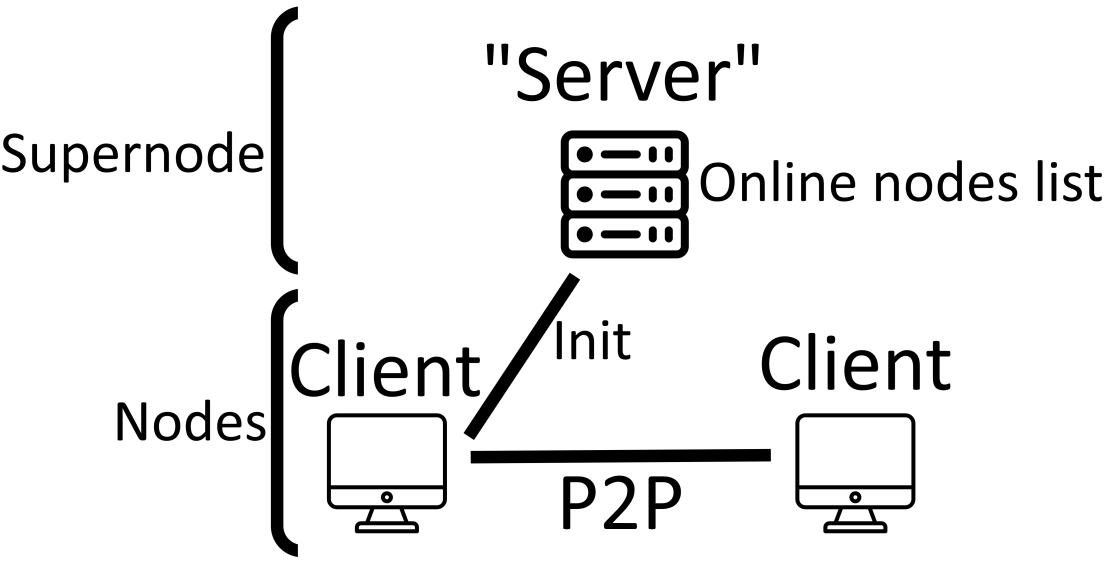
\includegraphics[width=0.8\linewidth]{report/schema-net.png}}
\end{center}

Le réseau est constitué de:
\begin{itemize}
    \item Supernodes: serveurs (ports ouverts) permettant aux nodes de communiquer entre elles.
    \item Nodes: clients
\end{itemize}

\subsection{Peer to peer (P2P)}

Une blockchain est basée sur la communication P2P entre les nodes.
Cependant, les clients utilisent la plupart du temps un routeur NAT dont les ports sont fermés.
Il faut donc des supernodes intermediaires afin d'initialiser une connection P2P.
On utilisera la méthode du hole punching pour ouvrir les ports des clients.

\subsection{Supernodes}

Les supernodes auront des addresses IP fixes, hardcodées dans la blockchain.
Il faut au minimum une supernode en ligne pour garantir le fonctionnement du réseau.
Les supernodes tiennent à jour une liste des nodes en ligne.
Toute initiation de connection P2P entre nodes se fait en passant par une supernode:
\begin{itemize}
    \item La node initiant la connection contacte la supernode pour obtenir l'addresse IP de la node visée
    \item Elle envoie ensuite un paquet à la cible, qui sera rejeté par le pare-feu. Cette étape a pour but d'ouvrir un port acceptant les paquets venant de la cible
    \item Elle envoie l'ID du port nouvellement ouvert à la supernode, qui le communique à la cible
    \item La cible envoie un paquet au port ouvert, qui cette fois est accepté
    \item Les 2 nodes ont à présent chacune un port ouvert acceptant les paquets venant de l'autre
\end{itemize}

\subsection{Messages}

Les paquets envoyés sur le réseau, appelés messages, possèdent une architecture prédéfinie.
Ils suivent l'architecture suivante:

\begin{table}[]
    \begin{tabular}{cc}
    \hline
    \multicolumn{1}{|c|}{\textbf{Bytes}} & \multicolumn{1}{c|}{\textbf{Valeur}}   \\ \hline
    \multicolumn{1}{|c|}{1}              & \multicolumn{1}{c|}{Magic (réseau)}    \\ \hline
    \multicolumn{1}{|c|}{1}              & \multicolumn{1}{c|}{Commande}          \\ \hline
    \multicolumn{1}{|c|}{4}              & \multicolumn{1}{c|}{Taille du contenu} \\ \hline
    \multicolumn{1}{|c|}{4}              & Hash du contenu                        \\
    \multicolumn{1}{|c|}{?}              & Contenu                               
    \end{tabular}
\end{table}

\section{Plateau de jeu}
Le jeu de billes est traditionnellement relié à l’univers des enfants et de l’école, nous nous sommes donc rapidement mis d’accord sur la nature du plateau de jeu : une cour de récréation.

\subsection{Première version 9,90 Mo}
Logiciels utilisés :
\begin{itemize}
    \item Google Sketchup 2017 (modélisation => export en .dae vers Blender)
    \item Blender 2.81 (export en .fbx vers Unity 2019.3.4
\end{itemize}

Cet environnement se compose d’une partie principale (la cour de récréation rectangulaire avec des grilles sur chaque face, un arbre d’un côté et l’école de l’autre) et d’une partie 	secondaire, le décor (un centre-ville de 70 buildings environ, plus d’une dizaine d’étages 	chacun). Le modèle est constitué presque exclusivement de composants originaux modélisés pour l’occasion, seul le bâtiment de l’école est un fichier téléchargé sur internet qui a été retravaillé ensuite pour l’incorporer dans le reste de la scène. Cette première version était finie fin janvier, sauf qu’au moment de l’incorporer au repo Git nous nous sommes rendus compte que le modèle était difficile à gérer dans Unity car la taille du fichier était beaucoup trop importante… le travail a donc été repris pour alléger le fichier.

\begin{figure}[htp] 
    \centering
    \subfloat{%
        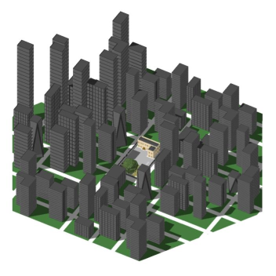
\includegraphics[width=0.3\linewidth]{report/building1.png}\\
        }%
    \hfill%
    \subfloat{%
        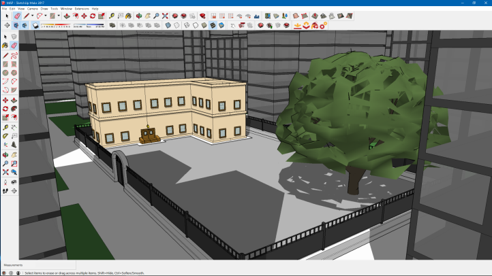
\includegraphics[width=0.6\linewidth]{report/map1.png}\\
        }%
\end{figure}

\subsection{Deuxième version 447,45 Ko}
Logiciels utilisés :
\begin{itemize}
    \item Google Sketchup 2017 (modélisation => export en .dae vers Blender)
    \item Blender 2.81 (export en .fbx vers Unity 2019.3.4
\end{itemize}

Cette deuxième version ne contient plus que la partie principale dénuée des grilles trop complexes (donc seulement la cour de récréation rectangulaire avec un arbre d’un côté et l’école de l’autre).

Elle fut finie début février, environ deux semaines après, et ne faisait plus que 4,8\% de sa taille 	originale (qui a engendré un gain considérable en performances).
Cette version requiert encore un peu de travail, surtout par rapport aux grilles qu’il va falloir 	remettre (en version simplifiée bien sûr).

\begin{center}
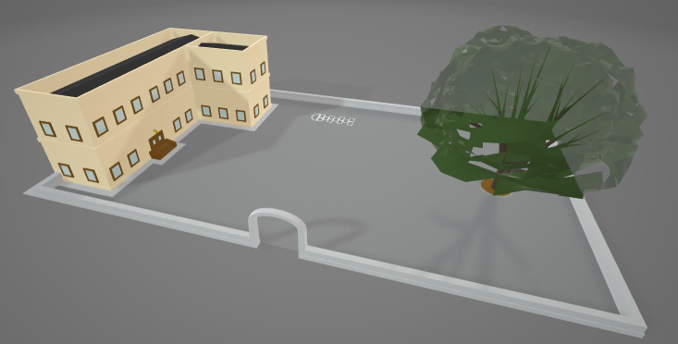
\includegraphics[width=0.8\linewidth]{report/map2.png}\\
\end{center}

\section{Design des billes}
C’est une partie du travail qui évolue lentement mais sûrement depuis le début du projet, et qui a (depuis fin février environ) atteint un stade assez satisfaisant pour qu’elle puisse être considéré comme temporairement terminée. Le jeu compte aujourd’hui six classes de billes, cinq d’entre elles correspondent chacune à cinq modèles différents (chaque modèle étant lui même disponible en six couleurs différentes), et la dernière classe étant la classe « spéciale » qui ne contient aujourd’hui qu’un modèle.

\subsection{Modèles 3D}
Logiciels utilisés :
\begin{itemize}
    \item Google Sketchup 2017 (modélisation => export en .dae vers Blender)
    \item Blender 2.81 (export en .fbx vers Unity 2019.3.4
\end{itemize}

Les modèles de billes actuels sont tous des modèles originaux créés pour l’occasion, un autre modèle de test avait été pris d’internet mais n’a pas pris place dans la collection finale.

\begin{center}
    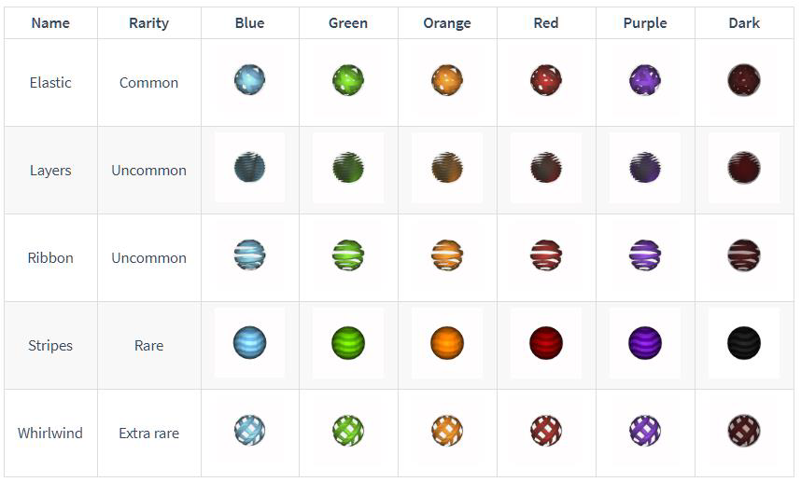
\includegraphics[width=0.8\linewidth]{report/marbles.png}\\
\end{center}

Les modèles « pèsent » respectivement 61 Ko, 210 Ko, 53 Ko, 127 Ko et 50 Ko (de haut en bas). Malgré les efforts qui ont été faits (et qui continuent d’être faits) pour rendre les 	ressources les plus légères possibles, certains modèles sont nettement plus lourds que les autres mais cela ne semble pour l’instant pas trop affecter les performances du jeu, ce n’est donc pas ici considéré comme un problème.

\subsection{Icônes}
Logiciels utilisés :
\begin{itemize}
    \item Double Commander 0.9.8 pour la normalisation des fichiers
    \item 3DBrowser 14.25 pour la génération des miniatures dans le format souhaité\\
\end{itemize}

Les fichiers 3D des billes ont d’abord reçu un traitement qui consistait à normaliser leurs noms (sous la forme « [modèle] - [couleur] »).
Ensuite, un deuxième traitement a été appliqué sur le groupe de fichiers : deux miniatures, une en .png (sur fond blanc) et l’autre en .gif (animation rotative antihoraire – 24 fps – fond blanc) ont été créées pour chaque bille.
Ces miniatures ont pu servir à l’élaboration d’un tableau inventaire animé qui viendra enjoliver le site internet, et serviront également sûrement pour les menus du jeu (un tableau de GIF est moins gourmand en ressources que le même tableau de fichiers 3D complets).


\section{Site web}
La construction du site web a été commencée par Aurèle. Il est fait en JavaScript, React.js et Sass.
Disponible à l'adresse \bold{www.scatteredcorp.tech}.\\[1ex]
\begin{center}
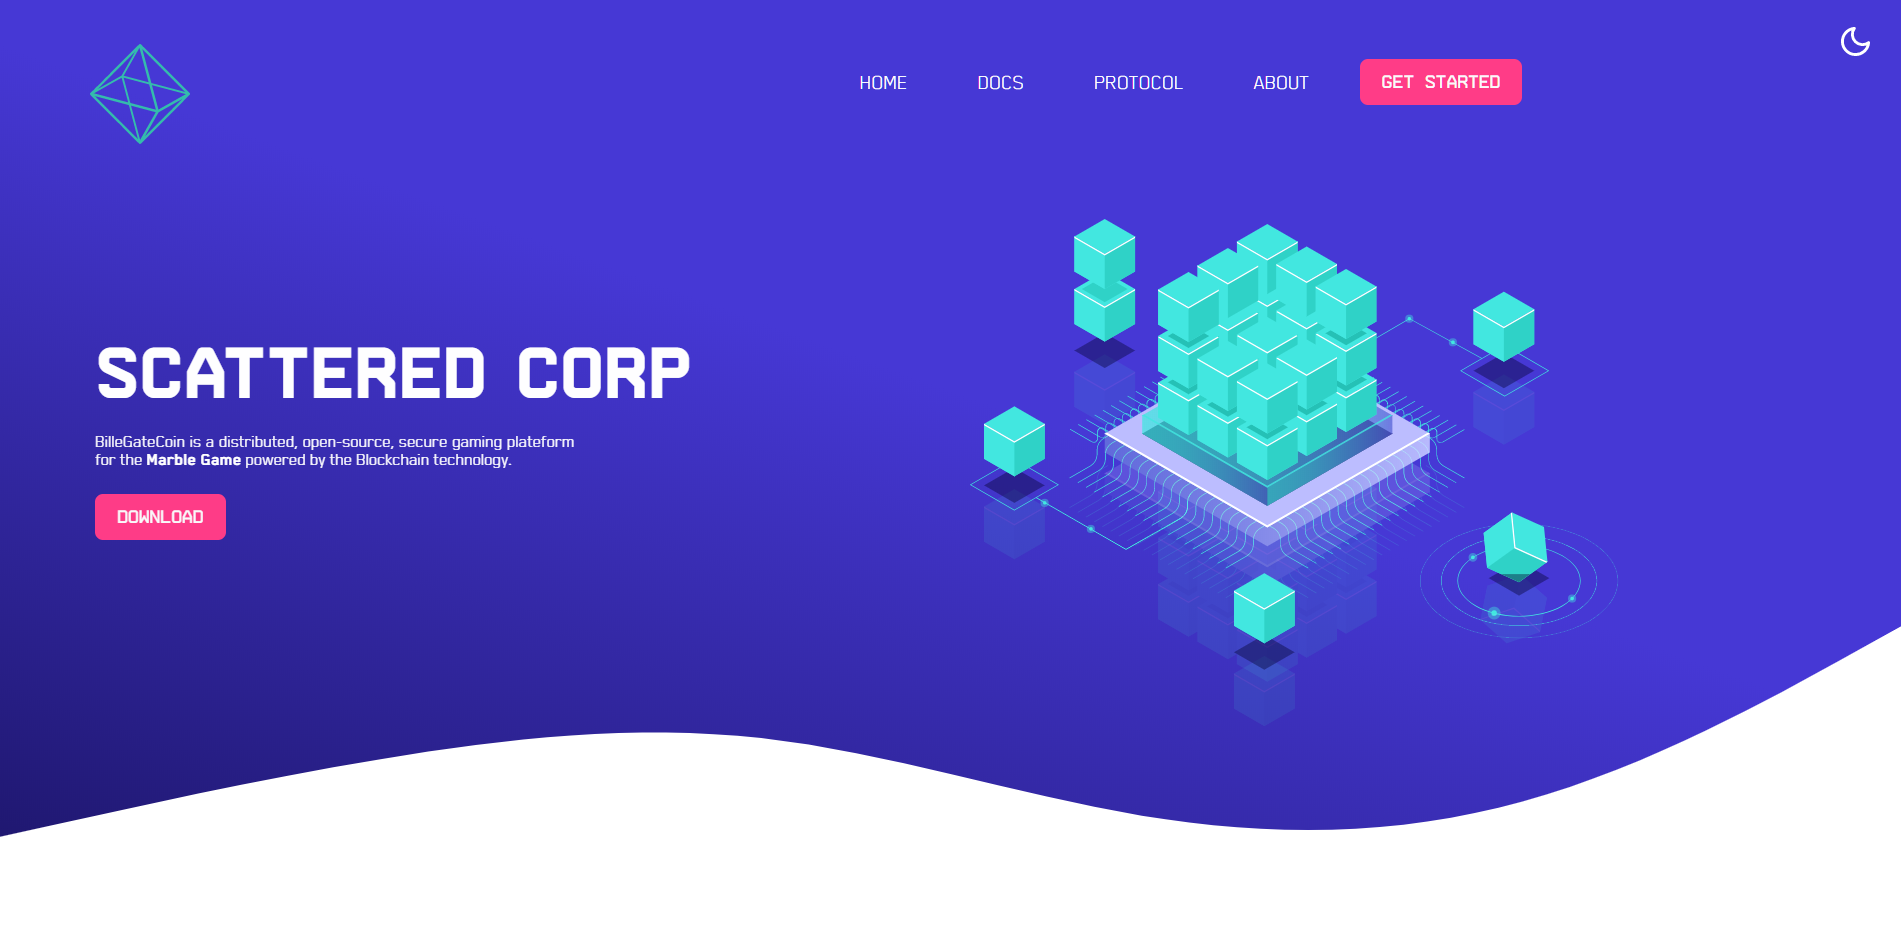
\includegraphics[width=0.8\linewidth]{report/website.png}\\
\end{center}

\section{Conclusion}
Le projet avance au rythme prévu et chaque membre est toujours aussi motivé.

\end{document}
